\documentclass[conference]{IEEEtran}
\IEEEoverridecommandlockouts
\usepackage{cite}
\usepackage{amsmath,amssymb,amsfonts}
\usepackage{graphicx}
\usepackage{booktabs}
\usepackage{array}
\usepackage{multirow}
\usepackage{xcolor}
\usepackage{url}
\graphicspath{{figures/}}

\begin{document}

\title{Ingredient Scanner: Noise-Robust Transformer-Based Named Entity Recognition for Detecting Hidden Ingredients in Food Packet Images}

% TODO: replace with the real author names, department and institution
\author{\IEEEauthorblockN{Author One}
\IEEEauthorblockA{\textit{Department of Computer Engineering} \\
\textit{Institution Name}\\
City, Country \\
email@example.com}
\and
\IEEEauthorblockN{Author Two}
\IEEEauthorblockA{\textit{Department of Computer Engineering} \\
\textit{Institution Name}\\
City, Country \\
email@example.com}
\and
\IEEEauthorblockN{Author Three}
\IEEEauthorblockA{\textit{Department of Computer Engineering} \\
\textit{Institution Name}\\
City, Country \\
email@example.com}
}

\maketitle

\begin{abstract}
Food labels often list sugars, fats and additives under unfamiliar names (dextrose, invert syrup, maltodextrin) or as numeric codes (INS/E~330), so shoppers cannot easily tell what a product contains. We present Ingredient Scanner, a system that takes a photo of a packet's ingredient list and returns every ingredient with its category, its function and any allergens. The pipeline combines optical character recognition (PP-OCRv6), dictionary-based spelling correction, a hybrid named entity recognizer (rules, a fine-tuned DistilBERT model and fuzzy knowledge-base matching) and entity linking to an additive knowledge base. Because hand-labelled data was not available, we trained on 22,323 Open Food Facts ingredient lists labelled automatically by rules (silver labels) across ten entity classes. To make the transformer robust to OCR errors, we inject synthetic character-confusion noise into half of the training sentences in every epoch. On text with 10\% OCR-style noise, the augmented DistilBERT reaches an entity-level F1 of 0.900, against 0.734 for the rule system, 0.796 for a CRF and 0.719 for DistilBERT trained without augmentation. On 60 real packet photos, the complete second version of the system raises the median share of ingredient words read from 0.72 to 0.96 and additive-identification F1 from 0.64 to 0.87 compared with our first version. We also report where the gains do not carry over: once OCR and spelling correction remove most character errors, the rule system remains slightly ahead on real photos when scored against rule-derived references. Finally, we compare our approach with the noise-aware training (NAT) method of Namysl et al.\ and build on it: we learn an OCR noise model from 39 real packet photos and add NAT's stability objective. Under an equal training budget, stability training gives the most noise-robust DistilBERT on every noisy test set (F1 0.813 against 0.758 without augmentation at 10\% noise), but the gain does not reach real photos, where the measured residual noise is only 2.3\% per character and most errors are missing text.
\end{abstract}

\begin{IEEEkeywords}
named entity recognition, DistilBERT, data augmentation, noise-aware training, optical character recognition, weak supervision, food labelling, food additives
\end{IEEEkeywords}

%=====================================================================
\section{Introduction}

Ingredient lists are the main source of information about what a packaged food contains, but they are hard to read. Small print, curved packaging and technical vocabulary all get in the way. Added sugar alone can appear under dozens of names, such as dextrose, glucose syrup, invert sugar or jaggery, and additives are often written only as numbers under the International Numbering System (INS) or the European E-number scheme~\cite{codex_ins}. A shopper who wants to limit free sugars, as recommended by the World Health Organization~\cite{who_sugars}, or to avoid a particular additive has to decode this vocabulary while standing in a shop.

We built Ingredient Scanner to do this decoding automatically. A user photographs the ingredient list; the system reads the text, finds every ingredient and explains it: which items are sugars or fats under another name, what each INS/E code means and what it is used for, and which of the 14 major allergen groups defined in EU Regulation 1169/2011~\cite{eu_1169} are present. A daily-intake guide compares a portion with published reference values. The system identifies and explains ingredients; it does not make health claims.

Two problems make this hard. First, there is no labelled dataset of food ingredient entities at the granularity we need (sugar, sweetener, fat, preservative, colour, additive, INS code, function class, flavouring, other ingredient). Second, the input comes from OCR, so the text the model sees is noisy: ``l'' becomes ``1'', ``O'' becomes ``0'', and ``dextrose'' becomes ``dextr0se''. A model trained on clean text from a product database may fail on text read from a photo.

This paper makes the following contributions:
\begin{itemize}
\item An end-to-end pipeline from packet photo to explained ingredients, combining OCR, spelling correction, a hybrid NER model and entity linking (Fig.~\ref{fig:pipeline}).
\item A silver-labelled corpus of 22,323 English ingredient lists from Open Food Facts~\cite{off}, with ten entity classes in BIO format, produced by weak supervision.
\item A comparison of six NER systems (dictionary rules, CRF, BERT, DistilBERT, DistilBERT with a CRF layer and DistilBERT with OCR-noise augmentation) under clean and noisy conditions, showing that noise augmentation is what makes the transformer robust.
\item An end-to-end evaluation on 60 real packet photos and 16 previously unseen products, including an honest account of where the deep learning gains do and do not transfer to real images.
\item A comparative analysis against noise-aware training (NAT)~\cite{namysl2020nat} (Section~\ref{sec:comparison}) and an extension of it: an OCR noise model learned from real packet photos and NAT's stability objective, evaluated on synthetic noise, learned noise and real photos (Section~\ref{sec:nat}).
\end{itemize}

%=====================================================================
\section{Related Work}

\textbf{Named entity recognition.} Sequence labelling for NER moved from feature-based conditional random fields (CRF)~\cite{crf} to neural models such as the BiLSTM-CRF~\cite{huang2015bilstm,lample2016neural}, and then to pretrained transformers. BERT~\cite{bert} fine-tunes a deep bidirectional encoder for token classification and set new results on standard NER benchmarks. DistilBERT~\cite{distilbert} compresses BERT by knowledge distillation, keeping about 97\% of its language-understanding performance while being 40\% smaller and 60\% faster, which matters for an application that must run on a CPU.

\textbf{Food information extraction.} The FoodBase corpus~\cite{foodbase} provides annotated food entities in recipe text, and rule-based systems such as FoodIE~\cite{foodie} extract food concepts from recipes. These resources target dishes and recipe ingredients rather than the regulatory vocabulary of packaged foods (additive codes, function classes such as ``acidity regulator'', hidden sugars), which is our focus.

\textbf{Weak supervision.} When hand labels are scarce, labels can be generated programmatically from heuristics and dictionaries. Snorkel~\cite{snorkel} formalised this idea. We follow the same principle with a single rule-based labeller built from curated lexicons and the Open Food Facts additive taxonomy, and we treat its output as silver rather than gold labels.

\textbf{Robustness to OCR noise.} Errors in OCR output degrade downstream NLP models. Namysl et al.~\cite{namysl2020nat} proposed noise-aware training for sequence labelling, augmenting training data with synthetic noise that imitates OCR and misspelling errors. Our augmentation follows this direction with a simple character-confusion model specific to label print; Section~\ref{sec:comparison} compares the two approaches in detail. For the OCR itself we use PP-OCR~\cite{ppocr}, a lightweight detection-and-recognition system, and for spelling correction the symmetric-delete algorithm SymSpell~\cite{symspell}.

%=====================================================================
\section{Base Paper and Comparative Analysis}
\label{sec:comparison}

We take the noise-aware training (NAT) paper of Namysl et al.~\cite{namysl2020nat} as our base paper, because it studies the same problem: sequence labelling models lose accuracy when their input contains OCR and spelling errors. NAT proposes two training methods. \emph{Data augmentation} adds noisy copies of the training sentences, generated by a noise model, to the training loss. \emph{Stability training} adds a term that penalises differences between the model's output distributions for a clean sentence and its noisy copy, so that noise should not change the prediction. NAT also argues that the noise model matters, and estimates realistic error distributions from the output of a real OCR engine instead of relying only on hand-designed errors.

Table~\ref{tab:comparison} compares NAT with our system as described in Sections~\ref{sec:dataset}--\ref{sec:results}. The two works agree on the central idea: robustness comes from exposing the model to noise during training. Our results confirm this for a different model family (a distilled transformer rather than a BiLSTM-CRF over contextual embeddings) and a new domain with its own vocabulary. They differ in three ways that matter. First, NAT uses gold-annotated benchmarks, while we train and evaluate on silver labels. Second, our original noise model is a set of 13 hand-picked character confusions, while NAT estimates its noise from real OCR output. Third, we use augmentation only, without the stability objective. On the other hand, our work evaluates a complete application on real photographs, which NAT does not attempt. The last two differences suggest a direct extension: estimate the noise from our own photos and add stability training. Section~\ref{sec:nat} does this.

\begin{table}[t]
\caption{Base paper (NAT) compared with our system}
\label{tab:comparison}
\centering
\footnotesize
\setlength{\tabcolsep}{3pt}
\begin{tabular}{>{\raggedright\arraybackslash}p{1.45cm}>{\raggedright\arraybackslash}p{3.1cm}>{\raggedright\arraybackslash}p{3.1cm}}
\toprule
Aspect & NAT~\cite{namysl2020nat} & Ingredient Scanner (ours) \\
\midrule
Domain & General news NER (English, German) & Food ingredient lists \\
Labels & Hand-annotated benchmarks & Silver (rule-generated) \\
Model & Contextual embeddings + BiLSTM-CRF & Fine-tuned DistilBERT \\
Noise model & Errors estimated from real OCR output & 13 hand-picked confusion pairs \\
Training & Augmentation and stability training & Augmentation only \\
Evaluation & Synthetic and OCR-generated noise & Synthetic noise and 60 real photos \\
Scope & Sequence labelling only & Full app: OCR to explanation \\
\bottomrule
\end{tabular}
\end{table}

%=====================================================================
\section{Dataset and Silver Labelling}
\label{sec:dataset}

\subsection{Source and Filtering}
We started from the full Open Food Facts export of 4,535,553 products, of which 72.4\% have no ingredient text. We kept products from English-speaking markets with a unique barcode, a non-empty ingredient list of 3--1,500 characters written in English, and removed exact duplicate lists (103,482 removed). From the remaining 405,812 products we sampled per market group to balance regions, giving 22,355 products: 7,000 from the UK and Ireland, 7,000 from North America, 4,355 from India and 4,000 from other English-speaking countries. Lists have a median length of 230 characters and about 14 comma-separated segments; 76.2\% contain brackets, 46.6\% contain percentages and 64.9\% contain at least one additive. The most frequent additive codes are 330 (citric acid), 471, 500, 322 and 551.

\subsection{Entity Schema and Silver Labels}
We defined ten entity classes: \texttt{SUGAR}, \texttt{SWEETENER}, \texttt{FAT}, \texttt{PRESERVATIVE}, \texttt{COLOUR}, \texttt{ADDITIVE}, \texttt{INS\_CODE}, \texttt{FUNCTION\_CLASS}, \texttt{FLAVOURING} and \texttt{INGREDIENT}. With BIO tagging this gives 21 tags. A rule-based labeller assigns these tags using curated lexicons (sugars, fats, sweeteners, flavourings, function classes), an additive alias list and the Open Food Facts additive taxonomy. Thirty-one records written mostly in non-Latin script and one over-long record were skipped, leaving 22,323 records with 1.40 million tokens and 357,934 entities (Table~\ref{tab:labels}). \texttt{INGREDIENT} dominates; \texttt{SWEETENER} and \texttt{PRESERVATIVE} are rare, appearing in 6.2\% and 10.9\% of products.

As a sanity check on the labeller, we compared the additive numbers it finds with those detected independently by Open Food Facts on the 3,487 test products. The two agree with precision 0.851, recall 0.912 and F1 0.881.

\begin{table}[t]
\caption{Silver label distribution (22,323 records)}
\label{tab:labels}
\centering
\begin{tabular}{lrr}
\toprule
Label & Entities & \% of products \\
\midrule
INGREDIENT & 211,986 & 95.8 \\
ADDITIVE & 32,811 & 49.6 \\
FUNCTION\_CLASS & 25,516 & 48.2 \\
SUGAR & 24,983 & 57.2 \\
FAT & 20,336 & 49.7 \\
INS\_CODE & 17,643 & 19.9 \\
FLAVOURING & 13,485 & 43.3 \\
COLOUR & 5,492 & 13.9 \\
PRESERVATIVE & 3,397 & 10.9 \\
SWEETENER & 2,285 & 6.2 \\
\midrule
Total & 357,934 & \\
\bottomrule
\end{tabular}
\end{table}

\subsection{Splits}
Products with the same name and brand were grouped (20,087 groups) so that near-duplicates never cross splits. The split is 15,556 training, 3,280 validation and 3,487 test records (69.7/14.7/15.6\%), with similar market mixes in each. To check for leakage, we computed for every validation and test product the highest Jaccard similarity between its ingredient segments and those of any training product: the median is 0.30, only 0.15\% of products reach 0.8 and none are identical.

\subsection{Real-Photo Test Sets}
For end-to-end evaluation we collected 60 packet photos of products held out from training, each paired with the product's typed ingredient list, and a further 16 photos of popular products not among those 60 (Nutella, Coca-Cola, KitKat, Maggi, Oreo, Haribo, Pringles and others). We also wrote expected results by hand for the typed lists of 15 popular products.

%=====================================================================
\section{Methodology}

\begin{figure*}[t]
\centering
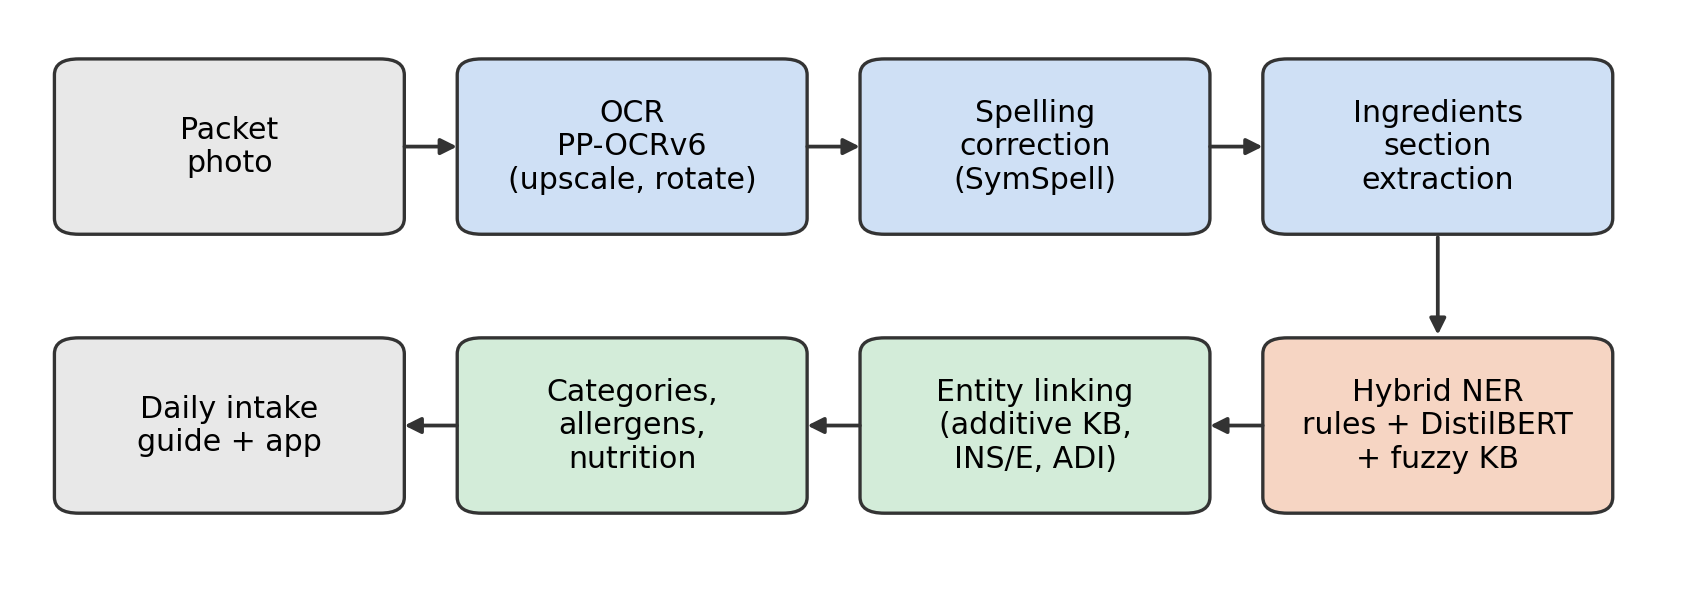
\includegraphics[width=0.72\textwidth]{fig_pipeline.png}
\caption{The Ingredient Scanner pipeline. Blue: text acquisition; orange: the hybrid NER model; green: interpretation.}
\label{fig:pipeline}
\end{figure*}

\subsection{OCR and Text Acquisition}
Our first version used EasyOCR and read a median of only 72\% of the ingredient words on our photos. The second version uses RapidOCR, an ONNX implementation of PP-OCRv6~\cite{ppocr}, with two pre-processing steps. Because ingredient print is often tiny, the photo is enlarged until the estimated text height is about 36 pixels. Because users photograph packets sideways or upside down, the orientation is chosen from the shape of the detected text boxes, confirmed by a quick recognition probe at four angles.

The OCR output then goes through three clean-up steps. A SymSpell~\cite{symspell} corrector repairs misspellings using a 6,800-word food dictionary built from the 22,000 real ingredient lists (for example ``maltodexirin'' $\rightarrow$ ``maltodextrin''). A code clean-up step repairs damaged additive codes (``33O'' $\rightarrow$ ``330''). Finally, the ingredient section is separated from the rest of the label (brand, nutrition table, storage text) by searching for an ``Ingredients'' keyword, falling back to the region with the highest density of commas, and finally to the full text.

\subsection{Hybrid Named Entity Recognition}
The recognizer combines three components in order of reliability:
\begin{enumerate}
\item \textbf{Exact rules}: dictionary and lexicon matches, which are precise for known spellings.
\item \textbf{DistilBERT}: a fine-tuned token classifier (Section~\ref{sec:distilbert}) that labels the spans the rules leave as generic or unknown, including misspelled words.
\item \textbf{Fuzzy knowledge-base matching}: remaining unknown spans are compared with the knowledge base using string similarity (rapidfuzz), so that near-misses can still be linked.
\end{enumerate}
Context rules handle constructions where the class is given by a neighbouring word, such as ``Colour (caramel)'' or ``Acidity regulator (INS~330)''. A statement filter removes text that is not an ingredient, such as allergy warnings (``Phenylketonurics: contains phenylalanine'').

\subsection{DistilBERT Fine-Tuning}
\label{sec:distilbert}
We fine-tuned \texttt{distilbert-base-uncased}~\cite{distilbert} with a linear token-classification head over the 21 BIO tags, using the Hugging Face Transformers library~\cite{wolf2020transformers}. Words are split into WordPiece sub-tokens, and only the first sub-token of each word carries the label; predictions are repaired afterwards so that every \texttt{I-} tag follows a matching \texttt{B-} or \texttt{I-} tag. The model minimises token-level cross-entropy, with non-first sub-tokens excluded from the loss. Training uses AdamW~\cite{adamw} with a learning rate of $5\times10^{-5}$, batch size 16, a linear schedule with 10\% warm-up, gradient clipping, a maximum length of 256 sub-tokens, two epochs and seed 42, on 8,000 training and 800 validation sentences. Batches are built from sentences of similar length to reduce padding. Training ran on a 4-core CPU in about 18 minutes.

We also trained three variants with the same budget: BERT-base-cased~\cite{bert} (learning rate $3\times10^{-5}$); DistilBERT with a CRF output layer, where the CRF transition parameters use a higher learning rate of $10^{-3}$; and DistilBERT with OCR-noise augmentation, described next. A feature-based linear-chain CRF~\cite{crf} serves as the classical baseline.

\subsection{OCR-Noise Augmentation}
OCR mostly fails by confusing characters that look alike. We model this with 13 confusion pairs, each applied in both directions: l/1, I/l, O/0, o/0, S/5, B/8, e/c, i/l, a/o, n/h, u/v, g/q and Z/2. Given a noise rate $r$, each character that has a confusion partner is replaced with probability $r$ by one of its partners:
\begin{equation}
\tilde{c}_i =
\begin{cases}
\text{random choice from } \mathcal{C}(c_i) & \text{with probability } r,\\
c_i & \text{otherwise,}
\end{cases}
\end{equation}
where $\mathcal{C}(c)$ is the set of confusion partners of character $c$. Labels are kept from the clean text, so the model learns to recover the correct class from damaged words. In every epoch, half of the training sentences receive fresh noise (character confusions or a change of letter case, since labels are often printed in capitals), so the model sees each sentence both clean and with different corruptions over training. Punctuation is not corrupted, so token boundaries and character offsets are preserved.

\subsection{Entity Linking and Interpretation}
Recognised entities are linked to a knowledge base of additives that maps INS/E numbers to names, function classes and acceptable daily intakes (ADI) from JECFA and EFSA. The output groups ingredients by category, highlights ``hidden'' items (sugars and fats under other names, additives written as codes, sugar-like carbohydrates such as maltodextrin), lists allergens as ``contains'' or ``may contain'', parses the nutrition table when present, and compares a chosen portion with WHO, EU and UK reference intakes. The result is shown in a Streamlit web application (Fig.~\ref{fig:app}).

%=====================================================================
\section{Experimental Setup}

\textbf{NER evaluation.} All systems are scored with the same strict entity-level micro F1: a prediction is correct only if both its span and label match the reference exactly. We evaluate on a 1,000-product sample of the silver test split (16,127 entities) under three conditions: clean text (\texttt{silver\_test}), and the same text with 5\% and 10\% character noise generated with the confusion model above (\texttt{noisy\_test\_0.05}, \texttt{noisy\_test\_0.10}). For the noisy sets the reference labels are those of the clean text. Because the silver labels are produced by the dictionary rules, the rule system scores 1.0 on clean text by construction; the noisy sets are therefore the more informative comparison.

\textbf{End-to-end evaluation.} On the 60 real photos we measure: the share of the typed list's ingredient words found in the OCR output (word recall); the character error rate (CER) of the extracted ingredient section; the number of readable photos (word recall $\geq 0.5$); entity F1 against the entities found in the typed list, with exact and fuzzy span matching; and precision, recall and F1 of the additive numbers identified, which is the question users care about most.

%=====================================================================
\section{Results}
\label{sec:results}

\subsection{Effect of OCR Noise on the Rule System}
Fig.~\ref{fig:noise} shows how the rule system degrades as noise increases. Its F1 falls from 1.0 on clean text to 0.969 at 1\% noise, 0.860 at 5\% and 0.738 at 10\%. The most affected classes are \texttt{ADDITIVE} (0.615 at 10\%) and \texttt{PRESERVATIVE} (0.622), whose long chemical names offer many characters to corrupt. This motivates a learned model that can recognise damaged words.

\begin{figure}[t]
\centering
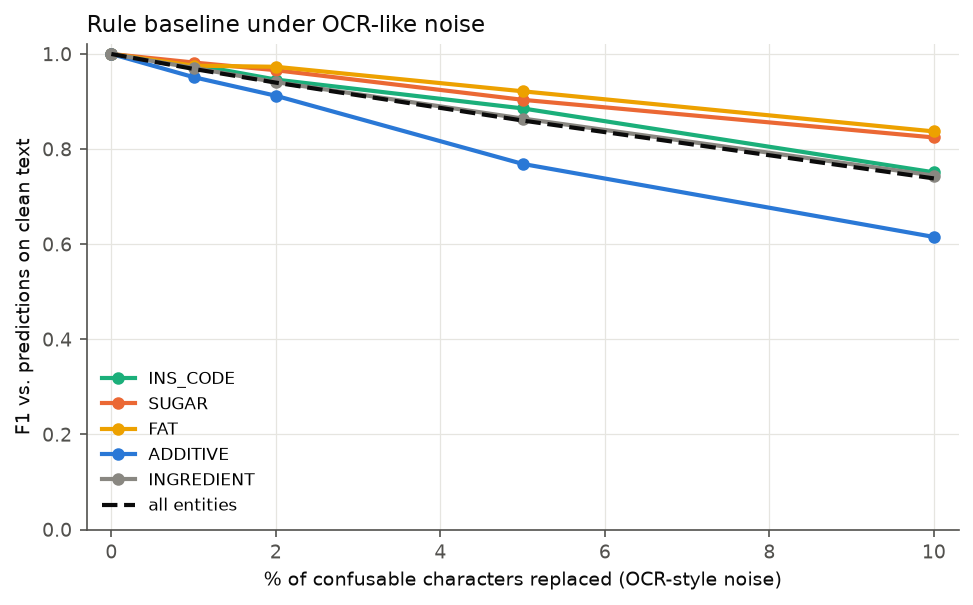
\includegraphics[width=0.8\columnwidth]{11_noise_robustness.png}
\caption{Entity-level F1 of the dictionary rules as synthetic OCR noise increases.}
\label{fig:noise}
\end{figure}

\subsection{NER Model Comparison and Ablation}
Table~\ref{tab:ner} and Fig.~\ref{fig:models} compare the six systems. On clean text all learned models reach 0.93--0.95, i.e.\ they reproduce the labelling policy well. Under noise the picture changes. Plain DistilBERT is no more robust than the rules (0.719 vs.\ 0.734 at 10\% noise), and neither BERT nor a CRF output layer closes the gap. With noise augmentation, DistilBERT keeps an F1 of 0.922 at 5\% and 0.900 at 10\% noise, 16.6 points above the rules and 10.4 points above the CRF, while losing only 0.3 points on clean text. The ablation shows that robustness comes from the training data rather than from model size or the output layer: BERT, which is larger, and the DistilBERT-CRF both perform worse than augmented DistilBERT under noise.

The cost is speed: the rules process 1,114 sentences per second and the CRF 664, against about 45 for DistilBERT and 14 for BERT on our CPU. For an app that classifies one ingredient list at a time, 45 sentences per second is more than enough.

\begin{table}[t]
\caption{Entity-level micro F1 of six NER systems. Speed in sentences per second on a 4-core CPU.}
\label{tab:ner}
\centering
\setlength{\tabcolsep}{4pt}
\begin{tabular}{lcccr}
\toprule
System & Clean & 5\% noise & 10\% noise & Speed \\
\midrule
Dictionary rules & 1.000$^\dagger$ & 0.862 & 0.734 & 1114 \\
CRF & 0.949 & 0.872 & 0.796 & 664 \\
BERT-base & 0.929 & 0.852 & 0.767 & 14 \\
DistilBERT & 0.943 & 0.834 & 0.719 & 47 \\
DistilBERT + CRF & \textbf{0.950} & 0.851 & 0.747 & 48 \\
DistilBERT + noise aug. & 0.940 & \textbf{0.922} & \textbf{0.900} & 45 \\
\bottomrule
\multicolumn{5}{l}{\footnotesize $^\dagger$Reference labels are produced by the rules.}
\end{tabular}
\end{table}

\begin{figure}[t]
\centering
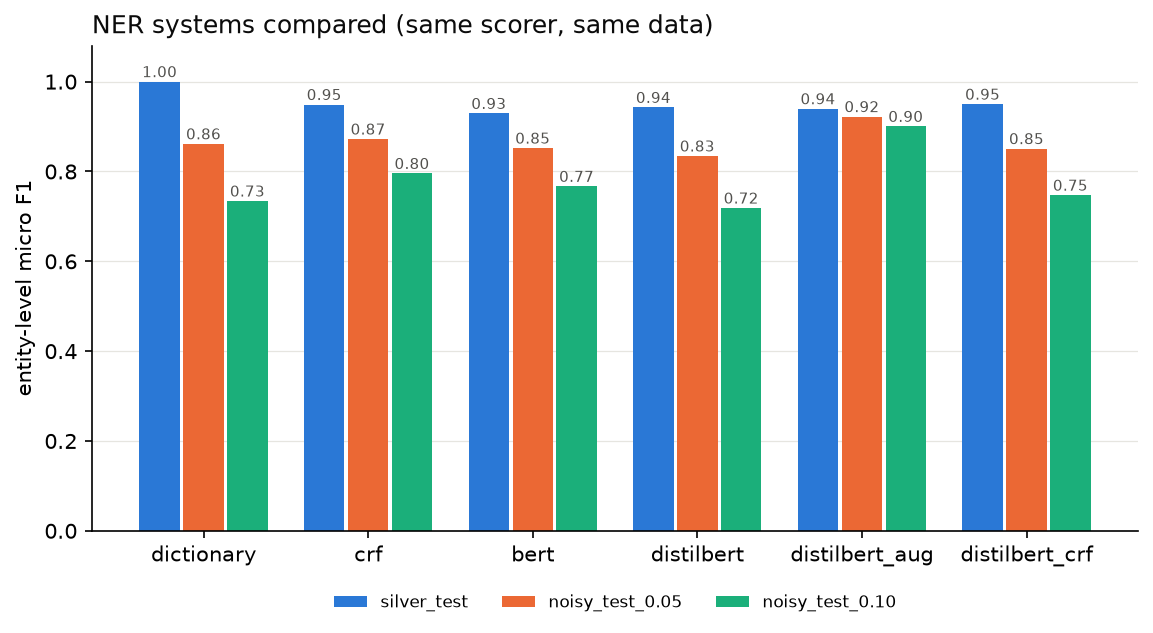
\includegraphics[width=\columnwidth]{12_model_comparison.png}
\caption{Entity-level micro F1 of all NER systems on clean and noisy silver test sets.}
\label{fig:models}
\end{figure}

Table~\ref{tab:perclass} shows per-class results for the augmented model at 5\% noise. Compared with the rules at the same noise level, the largest recall gains are for \texttt{ADDITIVE} (0.668 $\rightarrow$ 0.938), \texttt{INS\_CODE} (0.849 $\rightarrow$ 0.971) and \texttt{FUNCTION\_CLASS} (0.742 $\rightarrow$ 0.949). Precision drops somewhat, from 0.967 to 0.902 overall: the model accepts more damaged words, and some of them are wrong. \texttt{COLOUR} (F1 0.834) and \texttt{SWEETENER} (0.849, only 89 test entities) remain the weakest classes.

\begin{table}[t]
\caption{Per-class results of DistilBERT + noise augmentation at 5\% noise}
\label{tab:perclass}
\centering
\setlength{\tabcolsep}{4pt}
\begin{tabular}{lcccr}
\toprule
Class & P & R & F1 & Support \\
\midrule
SUGAR & 0.960 & 0.969 & 0.965 & 1150 \\
SWEETENER & 0.879 & 0.820 & 0.849 & 89 \\
FAT & 0.922 & 0.959 & 0.940 & 950 \\
PRESERVATIVE & 0.861 & 0.890 & 0.875 & 146 \\
COLOUR & 0.808 & 0.863 & 0.834 & 219 \\
ADDITIVE & 0.849 & 0.938 & 0.891 & 1444 \\
INS\_CODE & 0.832 & 0.971 & 0.896 & 697 \\
FUNCTION\_CLASS & 0.888 & 0.949 & 0.917 & 1091 \\
FLAVOURING & 0.887 & 0.917 & 0.902 & 581 \\
INGREDIENT & 0.914 & 0.941 & 0.927 & 9760 \\
\midrule
Micro average & 0.902 & 0.943 & 0.922 & 16127 \\
Macro F1 & & & 0.900 & \\
\bottomrule
\end{tabular}
\end{table}

Training was stable: the training loss fell from 0.523 after the first epoch to 0.133 after the second, and validation F1 rose from 0.929 to 0.944.

\subsection{End-to-End Results on Real Photos}
Table~\ref{tab:e2e} and Fig.~\ref{fig:v1v2} compare the first version of the system (EasyOCR, best NER model) with the second version (RapidOCR with enlargement and rotation, spelling correction, hybrid NER) on the same 60 photos. The median share of ingredient words read rose from 0.72 to 0.96, the number of readable photos from 42 to 55, and the CER of the extracted section fell from 0.64 to 0.22. Additive identification improved from F1 0.64 to 0.87, mainly through recall (0.48 $\rightarrow$ 0.82), and entity F1 with fuzzy matching from 0.52 to 0.77. Reading quality improved in every market; the largest gain was for the ``other English'' group, from 0.49 to 0.96.

\begin{table}[t]
\caption{End-to-end results on 60 real packet photos}
\label{tab:e2e}
\centering
\begin{tabular}{lcc}
\toprule
Metric & v1 & v2 \\
\midrule
Median word recall (full OCR) & 0.72 & \textbf{0.96} \\
Readable photos (of 60) & 42 & \textbf{55} \\
Median CER of ingredient section & 0.64 & \textbf{0.22} \\
Additives: precision & \textbf{0.97} & 0.92 \\
Additives: recall & 0.48 & \textbf{0.82} \\
Additives: F1 & 0.64 & \textbf{0.87} \\
Entity F1 (fuzzy match) & 0.52 & \textbf{0.77} \\
\bottomrule
\end{tabular}
\end{table}

\begin{figure}[t]
\centering
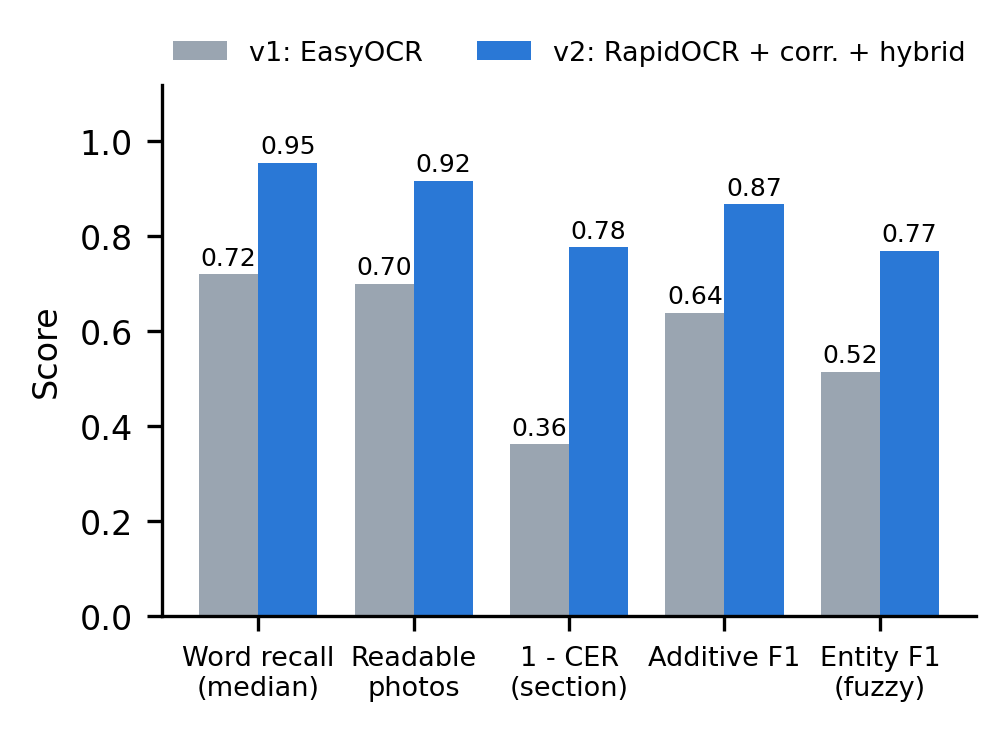
\includegraphics[width=0.8\columnwidth]{fig_v1_v2.png}
\caption{First (v1) and second (v2) system versions on the same 60 real photos.}
\label{fig:v1v2}
\end{figure}

How much of this gain is due to the NER model? Within each version we can compare NER systems on identical OCR output. With the noisier v1 OCR, augmented DistilBERT gave the best additive F1 (0.639, against 0.576 for the rules and 0.607 for plain DistilBERT). With the cleaner v2 OCR and spelling correction, however, the rule system is slightly ahead of the hybrid: additive F1 0.881 vs.\ 0.868 and fuzzy entity F1 0.794 vs.\ 0.770. We discuss this in Section~\ref{sec:discussion}.

\subsection{Unseen Products}
On the hand-checked typed lists of 15 popular products, the system found 100\% of the expected sugars, sweeteners, fats, preservatives and colours with no wrong extras, and 100\% of the expected additive codes with precision 0.94. On 16 new photos, compared with the result on each product's typed list, it recovered 56\% of category items and 60\% of additive codes. Flat, clear photos were read completely (both Nutella photos, KitKat Dark, Maggi sauce). Failures came from curved cans (Coca-Cola), labels where the list is small relative to the photo (Pringles), and multilingual packs where only part of the English text was visible (Oreo).

\begin{figure*}[t]
\centering
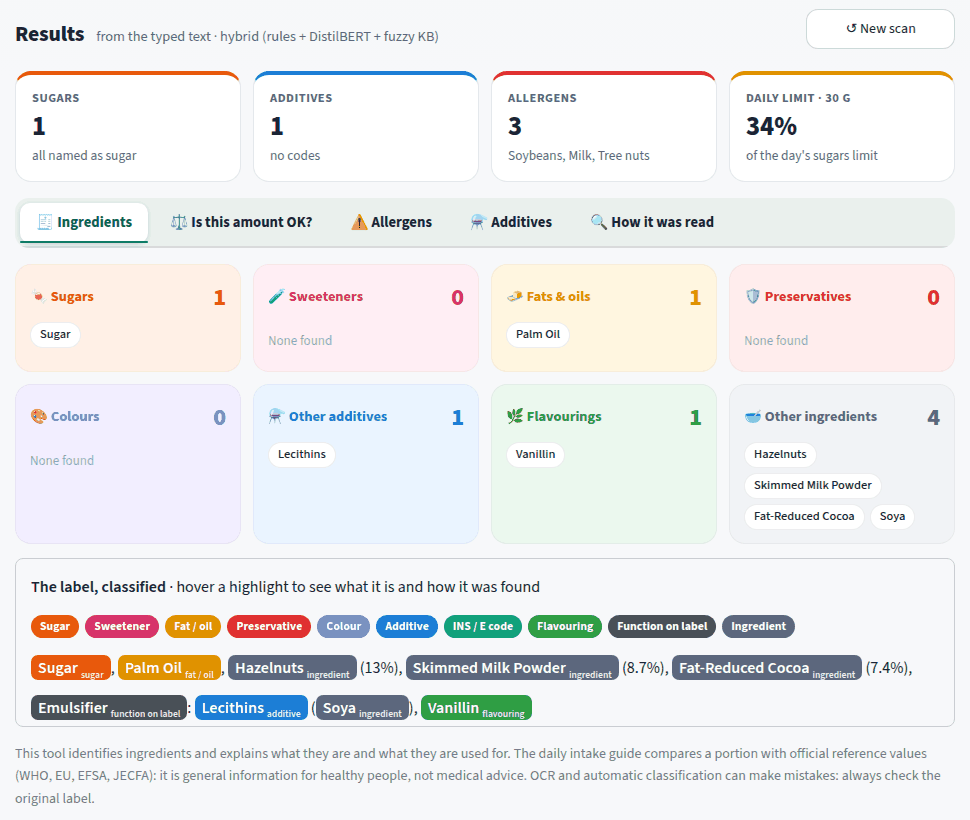
\includegraphics[height=3.9cm]{app_text_crop.png}\hfill
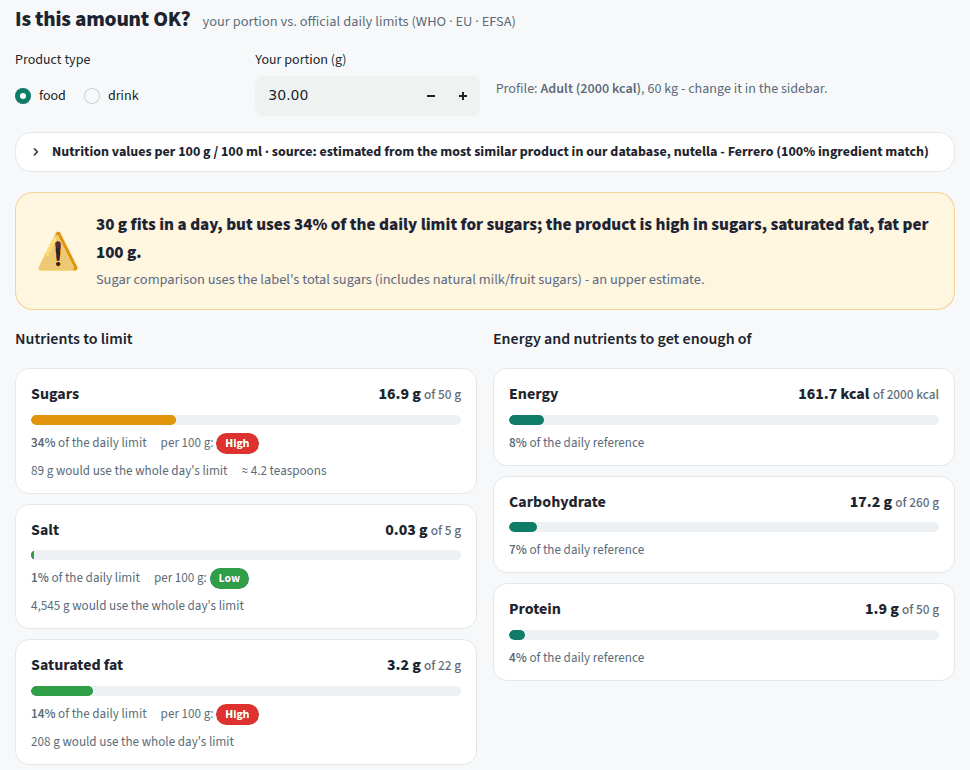
\includegraphics[height=3.9cm]{app_guide_crop.png}\hfill
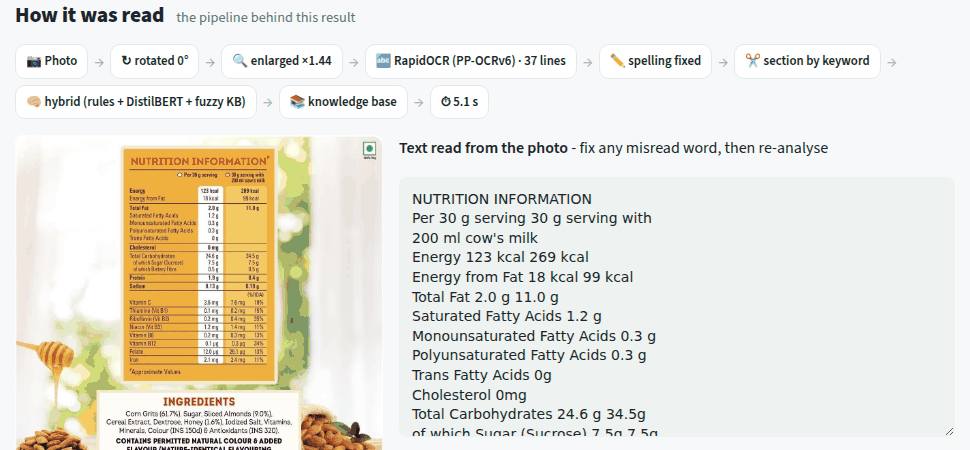
\includegraphics[height=3.9cm]{app_reading_crop.png}
\caption{The Streamlit application. Left: ingredients grouped by category, with each word of the label highlighted by its predicted class. Centre: daily intake guide for a 30\,g portion. Right: how a photo was read, from rotation and enlargement through OCR, spelling correction and the hybrid tagger.}
\label{fig:app}
\end{figure*}

%=====================================================================
\section{Extension: NAT-Style Training}
\label{sec:nat}

\subsection{Noise Model Learned from Real Photos}
Following NAT, we replaced the hand-picked confusions with errors measured on real data. For each of the 60 photos, we aligned the ingredient section that the app extracts (after OCR, code clean-up and SymSpell correction, i.e.\ exactly what the NER model receives) with the product's typed list, using a character-level Levenshtein alignment on lower-cased text. Photos whose aligned section differed too much from the typed list (similarity below 0.6, usually because the list is on a different panel or the product was reformulated) were skipped, leaving 39 photos and 8,444 reference letters and digits. Runs of three or more consecutive deleted or inserted characters were treated as missing or stray text rather than character errors: they cover 639 and 113 characters respectively and are counted but not simulated.

The remaining errors give per-character rates of 1.52\% substitutions, 0.62\% deletions and 0.14\% insertions, 2.3\% in total, with a separate substitution and insertion distribution for each character. The most frequent substitutions are l$\rightarrow$i, i$\rightarrow$l, t$\rightarrow$e and a$\rightarrow$o; a few, such as z$\rightarrow$s, reflect spelling variants between label and database (``stabilizer''/``stabiliser'') rather than OCR. Word merges (3.3 per 1,000 characters) and splits (0.8) were also counted but not simulated, so that the number of tokens, and therefore the labels, stay unchanged. The model corrupts each word independently: every character can be deleted, replaced by a character drawn from its own substitution distribution, or followed by an inserted character, each with its measured probability multiplied by a scale factor. At scale 1 it changes 7.2\% of the tokens of the test set, at scale 3 it changes 19.1\%.

\subsection{Stability Training}
NAT's stability objective pairs every training sentence $x$ with a noisy copy $\tilde{x}$ and minimises
\begin{equation}
\mathcal{L} = \mathcal{L}_{\mathrm{CE}}(x, y) + \alpha \sum_{i} \mathrm{KL}\big(p(y_i \mid x)\,\|\,p(y_i \mid \tilde{x})\big),
\end{equation}
where the sum runs over the words of the sentence (first sub-tokens). Because our noise keeps the word count unchanged, the $i$-th word of the clean copy always matches the $i$-th word of the noisy one. We use $\alpha=1$ and treat the clean distribution as a fixed target, so the gradient of the stability term only moves the prediction on the noisy copy. A fresh noisy copy is drawn for every sentence in every epoch; as in our augmentation, 60\% of copies receive learned noise (at 1$\times$, 2$\times$ or 4$\times$ the measured rate) and the rest a change of letter case.

\subsection{Setup}
We trained four DistilBERT models under an identical budget: 2,000 training sentences, two epochs, seed 42 and the hyperparameters of Section~\ref{sec:distilbert}. They differ only in the training regime: (a) no augmentation; (b) augmentation with the 13 hand-picked pairs, as in our main system; (c) augmentation with the learned noise; and (d) stability training with the learned noise. The budget is a quarter of that used in Section~\ref{sec:results}, because our CPU needed about 20 minutes per run and 39 minutes for stability training, which runs two forward passes per step. All systems were evaluated on the same 1,000 test products under five conditions: clean, 5\% and 10\% hand-picked noise, and learned noise at 1$\times$ and 3$\times$ its measured rate. The rules and the CRF from Section~\ref{sec:results} are included for reference; note that the CRF was trained on 8,000 sentences, four times as many as the DistilBERT models here.

\subsection{Results}
Table~\ref{tab:nat} and Fig.~\ref{fig:nat} show the results. Stability training gives the most robust DistilBERT on all four noisy test sets. At 10\% hand-picked noise it reaches 0.813, against 0.758 without augmentation and 0.805 with our original augmentation. On learned noise at 3$\times$ it reaches 0.814, against 0.767 and 0.795, and matches the CRF trained on four times the data. Two further results stand out. Augmentation with hand-picked pairs does not help at the realistic noise level (0.847 against 0.849 without augmentation on learned noise at 1$\times$), while learned noise does, slightly (0.854). And the learned-noise model trained without ever seeing the hand-picked confusions is almost as robust to them as the model trained on them (0.802 vs.\ 0.805 at 10\%). The differences among the three noise-trained models are small (0.4--1.0 points) and come from a single seed, so we read them as a consistent trend rather than a proven ranking.

\begin{table}[t]
\caption{Training regimes under an equal budget (2,000 sentences). Entity-level micro F1 on 1,000 test products.}
\label{tab:nat}
\centering
\footnotesize
\setlength{\tabcolsep}{2.0pt}
\begin{tabular}{lccccc}
\toprule
 & & \multicolumn{2}{c}{Pairs noise} & \multicolumn{2}{c}{Learned noise} \\
\cmidrule(lr){3-4}\cmidrule(lr){5-6}
System & Clean & 5\% & 10\% & 1$\times$ & 3$\times$ \\
\midrule
Dictionary rules & 1.000$^\dagger$ & 0.862 & 0.734 & 0.888 & 0.707 \\
CRF (8,000 sent.) & 0.949 & 0.872 & 0.796 & 0.899 & 0.814 \\
\midrule
(a) DistilBERT & \textbf{0.888} & 0.827 & 0.758 & 0.849 & 0.767 \\
(b) + pairs aug. & 0.877 & 0.839 & 0.805 & 0.847 & 0.795 \\
(c) + learned aug. & 0.881 & 0.841 & 0.802 & 0.854 & 0.804 \\
(d) + NAT stability & 0.880 & \textbf{0.847} & \textbf{0.813} & \textbf{0.858} & \textbf{0.814} \\
\bottomrule
\multicolumn{6}{l}{\scriptsize Bold: best DistilBERT. $^\dagger$Reference labels come from the rules.}
\end{tabular}
\end{table}

\begin{figure}[t]
\centering
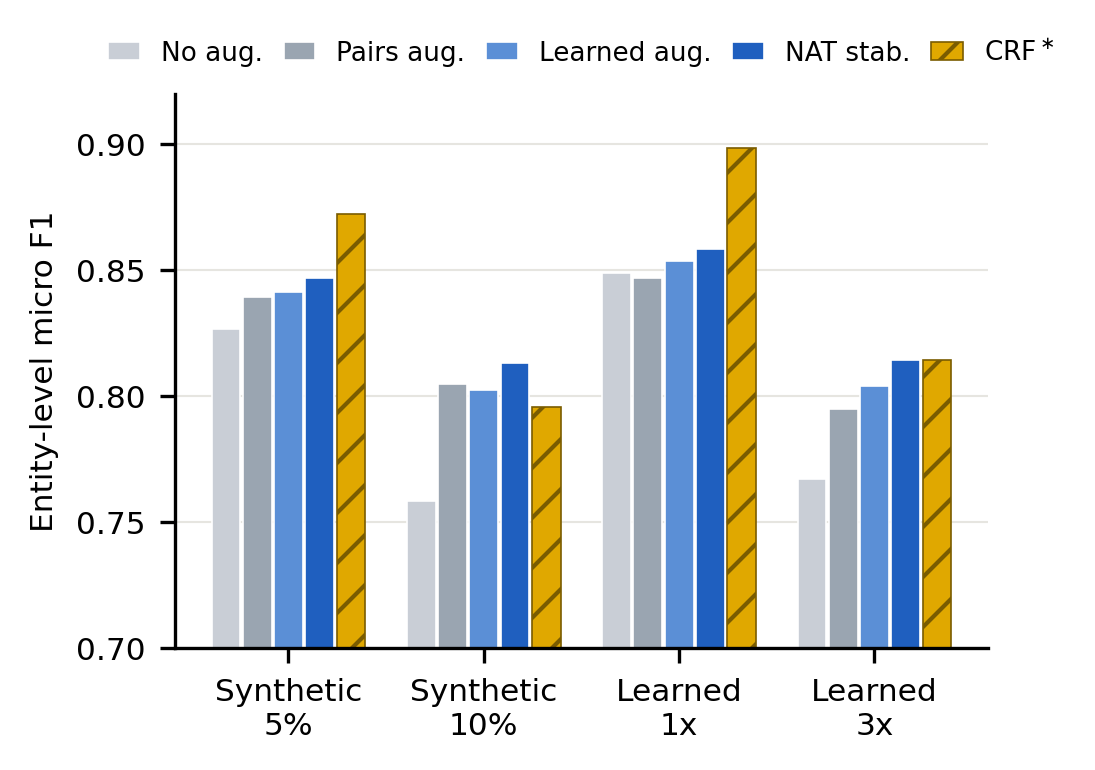
\includegraphics[width=0.95\columnwidth]{fig_nat_comparison.png}
\caption{Robustness of the four training regimes on noisy test sets. $^\ast$The CRF was trained on four times as many sentences.}
\label{fig:nat}
\end{figure}

Per class, the learned-noise models improve most on \texttt{SUGAR} (0.774 $\rightarrow$ 0.840 F1 at 3$\times$ learned noise with stability training) and \texttt{ADDITIVE} (0.620 $\rightarrow$ 0.706). They remain weak on the rare classes, where 2,000 sentences provide few examples: \texttt{SWEETENER} scores 0.20--0.29 and \texttt{COLOUR} 0.36--0.43 for every DistilBERT variant, against 0.70 and 0.71 for the CRF. Most of the CRF's lead on the realistic test set comes from these classes.

\subsection{Real Photos}
On the 60 real photos (Table~\ref{tab:natphoto}), the differences between the four regimes nearly disappear: fuzzy entity F1 ranges from 0.750 to 0.756 and additive F1 from 0.830 to 0.850, with the unaugmented model slightly ahead on additives. The rules remain best (0.795 and 0.881). This matches what the noise model itself shows: after OCR and spelling correction, only 2.3\% of characters are wrong, and more text is lost through missing spans than through character errors. A training method that makes the tagger robust to character errors therefore has little left to fix on our photos. NAT-style training is most useful where character noise is high, as with our first OCR engine or with harder photos; on our current pipeline, the next gains must come from reading more of the text, not from tagging damaged words better.

\begin{table}[t]
\caption{Training regimes on the 60 real photos}
\label{tab:natphoto}
\centering
\footnotesize
\begin{tabular}{lcc}
\toprule
System & Entity F1 (fuzzy) & Additive F1 \\
\midrule
Dictionary rules & \textbf{0.795} & \textbf{0.881} \\
CRF (8,000 sent.) & 0.778 & 0.857 \\
Hybrid (app, Section~\ref{sec:results}) & 0.770 & 0.868 \\
\midrule
(a) DistilBERT, no aug. & 0.756 & 0.850 \\
(b) + pairs aug. & 0.751 & 0.830 \\
(c) + learned aug. & 0.750 & 0.834 \\
(d) + NAT stability & 0.756 & 0.838 \\
\bottomrule
\end{tabular}
\end{table}

%=====================================================================
\section{Discussion and Error Analysis}
\label{sec:discussion}

The results tell a consistent story: the transformer helps in proportion to how noisy its input is. On synthetic noise and on the noisier v1 OCR, noise-augmented DistilBERT clearly beats the rules. In v2, better OCR and SymSpell correction already repair most character confusions before the NER step, so the advantage that augmentation gives shrinks. Two further effects work against the model on real photos. First, the remaining errors are mostly not character confusions but segmentation problems (words merged across lines, a wrong section boundary, missing lines), which our noise model does not simulate. Second, the end-to-end references are entities found in the typed list, and the per-class F1 is measured against silver labels, both of which follow the rule system's labelling policy; any genuine improvement by the model that disagrees with the rules is counted as an error.

We categorised all 1,747 errors of the augmented model on the 5\% noise set: 824 false positives (47\%), 322 boundary errors, 251 false negatives, 213 type errors and 137 errors of both boundary and type. The excess of false positives matches the precision drop in Table~\ref{tab:perclass}. Many \texttt{INS\_CODE} errors are boundary disagreements over code variants: the model tags ``INS~500~ii'' as one entity where the silver reference tags ``INS~500'' and ``ii'' separately, and it also tags bare numbers in brackets after a function class (``vegetable gum (414)'') that the rules leave unlabelled. Arguably, several of these are correct and the reference is wrong. \texttt{COLOUR} errors come from multi-word colour names broken by noise (``yeIlow 5 lakc'') and from overlap between categories, such as a damaged ``titanium dioxide'' predicted as a preservative. \texttt{SWEETENER} has only 89 test entities, so its scores are the least reliable.

On real photos, the dominant failure is OCR, not NER: when the ingredient words are not read, no tagger can recover them. The five unreadable photos and most misses on the 16 unseen products come from curvature, glare, very small print and mixed-language panels. For such photos the application warns the user and offers rotate, crop and text-correction tools.

%=====================================================================
\section{Limitations and Ethics}

\textbf{Silver evaluation.} All NER scores use rule-generated references, which favour the rule system. A gold-standard set of 480 sentences has been sampled for annotation by three annotators, but the annotation was not complete at the time of writing; gold-set results would give a fairer comparison between systems.

\textbf{Noise models.} Both noise models change characters within words only. The learned model is estimated from 39 photos, so rare characters fall back to global rates, and it does not simulate the word merges and missing spans that cause most real losses.

\textbf{Extension budget.} The NAT experiments use 2,000 training sentences and a single seed because of CPU time. Differences below about one point between the noise-trained models should be confirmed with more data and several seeds.

\textbf{Language and coverage.} The system handles English lists only, and the photo sets are small (60 and 16 photos). Products from India, the UK, North America and other English-speaking markets are included, but other regions are not.

\textbf{Ethics.} The system identifies ingredients and explains what they are and what they are used for. It does not label products as healthy or unhealthy. The intake guide quotes cited reference values for healthy adults, and the application states that this is general information, not medical advice, and that OCR and classification can make mistakes, so users should check the original label, especially for allergens.

%=====================================================================
\section{Conclusion and Future Work}

We presented Ingredient Scanner, a pipeline that reads food ingredient lists from photos and explains hidden sugars, fats, additives and allergens. Training DistilBERT on silver labels with OCR-style noise augmentation made it far more robust to character errors than rules, a CRF, BERT or DistilBERT without augmentation, raising entity F1 at 10\% noise from 0.734 to 0.900. Together with better OCR and spelling correction, the complete system raised additive identification on real photos from F1 0.64 to 0.87.

Building on noise-aware training, we learned an OCR noise model from real packet photos and added NAT's stability objective. Under an equal budget, stability training produced the most robust DistilBERT on every noisy test set, while hand-picked noise did not help at the realistic noise level. The measured noise also explains why none of these gains reach real photos: after correction, only 2.3\% of characters are wrong, and missing text dominates.

Our results show that the benefit of a robust model depends on how noisy its input is, and that the main remaining errors on real photos come from OCR and section segmentation. Future work will (i) complete the gold annotation and evaluate all systems on it; (ii) extend the learned noise model to word merges and missing spans, and repeat the NAT experiments with the full training set and several seeds; (iii) replace the rule-based section finder with a learned line classifier; (iv) train a multilingual model such as XLM-RoBERTa for multilingual packs; and (v) fine-tune the OCR recognizer on label crops.

\section*{Acknowledgment}
Product data comes from Open Food Facts, released under the Open Database License. % TODO: add any AI-tool use your course requires you to disclose.

\begin{thebibliography}{00}
\bibitem{codex_ins} Codex Alimentarius Commission, ``Class names and the International Numbering System for food additives,'' CAC/GL 36-1989, FAO/WHO.
\bibitem{who_sugars} World Health Organization, \textit{Guideline: Sugars Intake for Adults and Children}. Geneva: WHO, 2015.
\bibitem{eu_1169} European Parliament and Council, ``Regulation (EU) No 1169/2011 on the provision of food information to consumers,'' \textit{Official Journal of the European Union}, L 304, pp. 18--63, 2011.
\bibitem{off} Open Food Facts, ``Open Food Facts: the free food products database.'' [Online]. Available: \url{https://world.openfoodfacts.org}
\bibitem{crf} J. Lafferty, A. McCallum, and F. Pereira, ``Conditional random fields: Probabilistic models for segmenting and labeling sequence data,'' in \textit{Proc. ICML}, 2001, pp. 282--289.
\bibitem{huang2015bilstm} Z. Huang, W. Xu, and K. Yu, ``Bidirectional LSTM-CRF models for sequence tagging,'' arXiv:1508.01991, 2015.
\bibitem{lample2016neural} G. Lample, M. Ballesteros, S. Subramanian, K. Kawakami, and C. Dyer, ``Neural architectures for named entity recognition,'' in \textit{Proc. NAACL-HLT}, 2016, pp. 260--270.
\bibitem{bert} J. Devlin, M.-W. Chang, K. Lee, and K. Toutanova, ``BERT: Pre-training of deep bidirectional transformers for language understanding,'' in \textit{Proc. NAACL-HLT}, 2019, pp. 4171--4186.
\bibitem{distilbert} V. Sanh, L. Debut, J. Chaumond, and T. Wolf, ``DistilBERT, a distilled version of BERT: smaller, faster, cheaper and lighter,'' arXiv:1910.01108, 2019.
\bibitem{foodbase} G. Popovski, B. Korou\v{s}i\'{c} Seljak, and T. Eftimov, ``FoodBase corpus: a new resource of annotated food entities,'' \textit{Database}, vol. 2019, baz121, 2019.
\bibitem{foodie} G. Popovski, S. Kochev, B. Korou\v{s}i\'{c} Seljak, and T. Eftimov, ``FoodIE: A rule-based named-entity recognition method for food information extraction,'' in \textit{Proc. ICPRAM}, 2019, pp. 915--922.
\bibitem{snorkel} A. Ratner, S. H. Bach, H. Ehrenberg, J. Fries, S. Wu, and C. R\'{e}, ``Snorkel: Rapid training data creation with weak supervision,'' \textit{Proc. VLDB Endowment}, vol. 11, no. 3, pp. 269--282, 2017.
\bibitem{namysl2020nat} M. Namysl, S. Behnke, and J. K\"{o}hler, ``NAT: Noise-aware training for robust neural sequence labeling,'' in \textit{Proc. ACL}, 2020, pp. 1501--1517.
\bibitem{ppocr} Y. Du \textit{et al.}, ``PP-OCR: A practical ultra lightweight OCR system,'' arXiv:2009.09941, 2020.
\bibitem{symspell} W. Garbe, ``SymSpell: Symmetric delete spelling correction algorithm,'' 2012. [Online]. Available: \url{https://github.com/wolfgarbe/SymSpell}
\bibitem{wolf2020transformers} T. Wolf \textit{et al.}, ``Transformers: State-of-the-art natural language processing,'' in \textit{Proc. EMNLP: System Demonstrations}, 2020, pp. 38--45.
\bibitem{adamw} I. Loshchilov and F. Hutter, ``Decoupled weight decay regularization,'' in \textit{Proc. ICLR}, 2019.
\end{thebibliography}

\end{document}
